\documentclass[twoside]{article}
\usepackage{graphicx}
\usepackage{polski}
\usepackage{fancyhdr}
\usepackage{lastpage}
\usepackage{listings}
\usepackage{soul}
\usepackage{color}
\usepackage{multirow}
\usepackage{subcaption}

\title{AiSD Ex. 0 (Wszyscy)}
\author{\hl{Mateusz Kamieniecki}}
\date{\today}

\lstset{basicstyle=\ttfamily}

\makeatletter

\begin{document}

\pagestyle{fancy}
\fancyhead{}
\fancyhead[L]{\@title}
\fancyhead[R]{\@author}
\fancyhead[C]{\@date}

\cfoot{\thepage\ / \pageref{LastPage}}


\newpage

\section{Wprowadzenie}

Dzisiaj jest ten dzień, gdy rozpoczynamy nowe zajęcia.
Jeśli dotarliśmy do tego momentu, to oznacza, że kwestie organizacyjne mamy już za sobą.
Czy na pewno?

W trakcie tego semestru, jak zawsze, będziemy pracować w pewnym rygorze czasowym, ale dodatkowo
będziemy musieli przestrzegać kilku zasad, aby prawidłowo oddać pracę do oceny.

Ten dokument (jak i każdy kolejny w trakcie semestru) w formie wynikowej (PDF) należy wgrać 
do ISOD-a przed końcem zajęć.

Dodatkowo cały kod (w formie źródłowej, bez zbędnych zależności) należy umieścić w wydziałowym repozytorium Git-a, dostępnym z ISOD-a.

Wynikowe zmiany, zgodnie z poleceniem przy każdym ćwiczeniu, należy oznaczać konkretnymi tagami
(ze znacznikiem czasowym).

Brzmi groźnie?
To nic wielkiego.
Jest kilka poleceń, których musimy się nauczyć. 
A w razie problemów z pamięcią będziemy mogli sięgnąć do tego dokumentu.

Czy to zawsze zadziała?
Absolutnie nie!
Jeśli bardzo namieszamy, to te podstawowe polecenia nam nie wystarczą.

I co wtedy?
Wtedy ktoś musi schować się w budce telefonicznej, założyć niebiesko-czerwony kostium i ruszyć
z pomocą.
Miejmy jednak nadzieję, że unikniemy tych sytuacji.
Wystarczy, że...

\subsection{Fantastycznie podstawowe polecenia Git-a i jak je znaleźć}

Poniżej mamy spisanych kilka kroków, które są niezbędne, żeby nasza praca przebiegła pomyślnie i bez większych problemów.

\subsubsection{Klonowanie repozytorium}

W ISOD-zie, w miejscu z ocenami do naszych zajęć laboratoryjnych, znajdziemy niebieski przycisk 
\textit{Przejdź do Projektora} (rys. \ref{fig:projektor_isod_przycisk}).

\begin{figure}
    \centering
    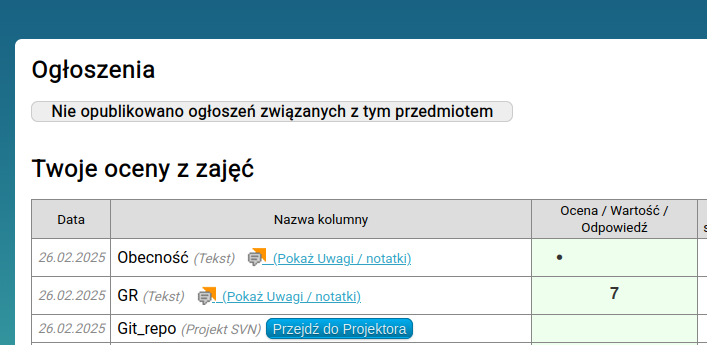
\includegraphics[width=1\linewidth]{images/projektor/Projektor_1.png}
    \caption{Gdzie znaleźć przycisk \textit{Przejdź do Projektora}?}
    \label{fig:projektor_isod_przycisk}
\end{figure}

Po kliknięciu (\textit{Przejdź do Projektora}) w przeglądarce powinna otworzyć się oczekiwana
strona.
Niestety ze względów niezależnych od nas (Wydziału) to połączenie jest szyfrowane, ale nie ma
aktualnego certyfikatu.
Dlatego, zamiast oczekiwanej strony \textit{Projektora}, wyświetli się strona informująca nas
o zagrożeniu (rys. \ref{fig:projektor_brak_certyfikatu}) 
i ryzyku, które podejmujemy, ignorując to ostrzeżenie 
(rys. \ref{fig:projektor_akceptowanie_ryzyka}).

\begin{figure}
    \centering
    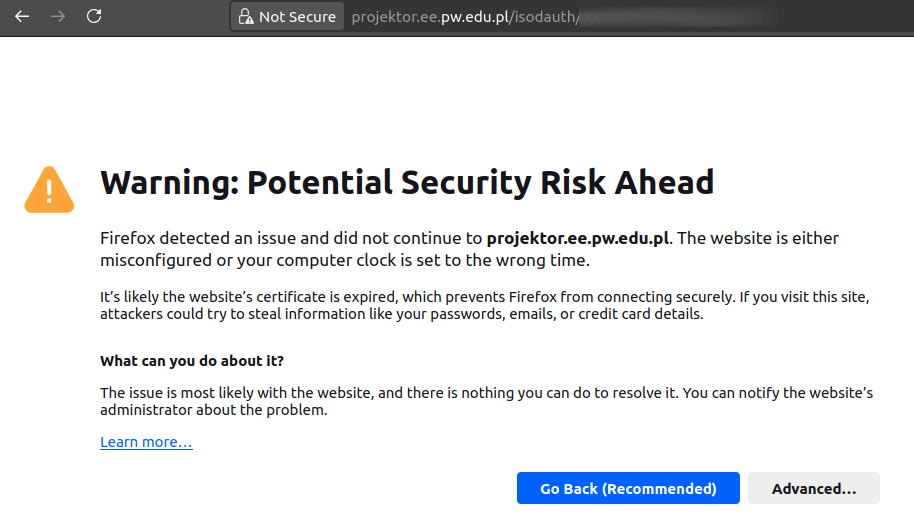
\includegraphics[width=1\linewidth]{images/projektor/Projektor_2.png}
    \caption{Ostrzeżenie o ryzyku ze względu na brak certyfikatu.}
    \label{fig:projektor_brak_certyfikatu}
\end{figure}

\begin{figure}
    \centering
    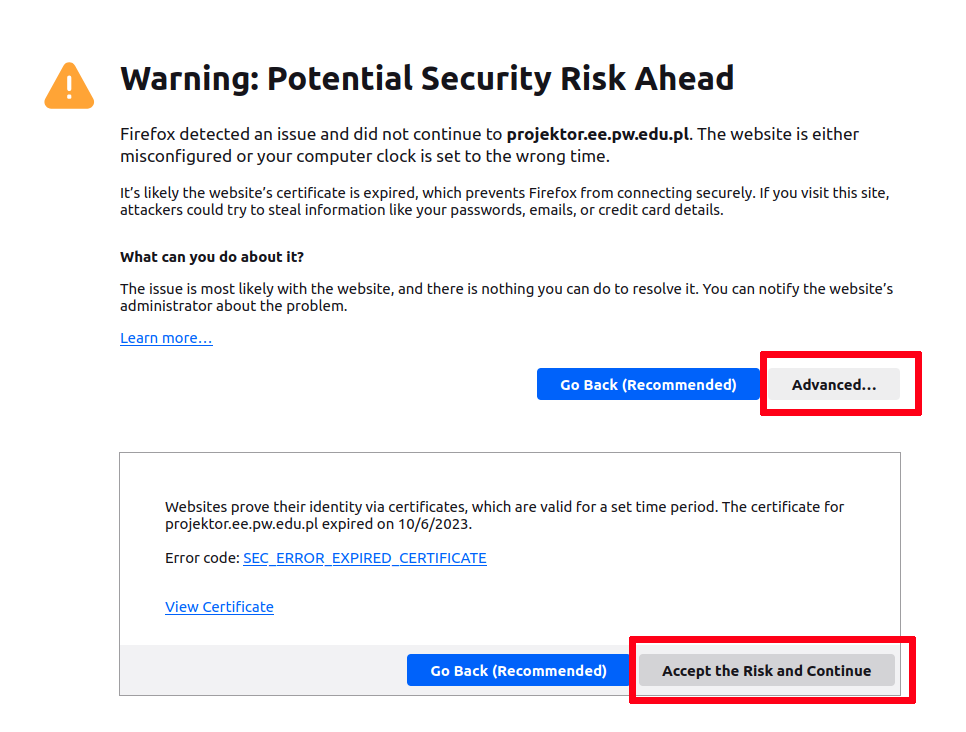
\includegraphics[width=1\linewidth]{images/projektor/Projektor_3.png}
    \caption{Zaakceptowanie ryzyka braku aktualnego certyfikatu.}
    \label{fig:projektor_akceptowanie_ryzyka}
\end{figure}

Jeśli to, co powyżej, mamy już za sobą, to teraz będzie już tylko trudniej.

Na nowo otwartej stronie próbujemy odszukać link zaczynający się od \verb|https://| 
(rys. \ref{fig:projektor_landing_page}).
(Uwaga dla chętnych: można też wybrać wersję z \verb|ssh|, ale to będzie wymagało podania klucza publicznego. Projektor ogranicza nas do jednego klucza, czyli jednej maszyny.)
Klikamy ,,w niego'', co skutkuje otwarciem strony \textit{401 Unauthorized}.
Ignorujemy (domyślny) formularz logowania, a następnie z adresu przeglądarki kopiujemy 
zawartość (cały adres).

\begin{figure}
    \centering
    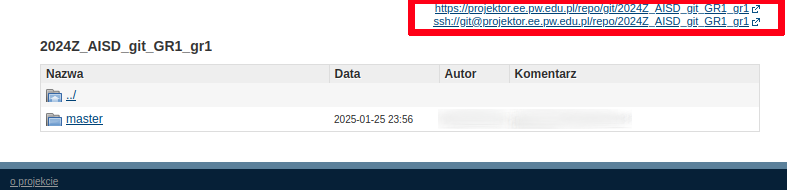
\includegraphics[width=1\linewidth]{images/projektor/Projektor_4.png}
    \caption{Widok \textit{Projektora} ze wskazaniem adresów do klonowania repozytorium.}
    \label{fig:projektor_landing_page}
\end{figure}

Naszym kolejnym krokiem jest wybranie lokalizacji na dysku, gdzie będziemy chcieli sklonować
repozytorium.
Otwieramy w tym miejscu terminal (w przypadku MS Windows szczerze polecam konsolę \textit{GitBash}).
Gdy już jesteśmy ustawieni w docelowym miejscu wykonujemy:

\begin{lstlisting}[frame=single,language=bash] 
git clone -c http.sslVerify=false <skopiowany_adres>
\end{lstlisting}

Warto zwrócić uwagę na flagę \verb|-c http.sslVerify=false| -- dodajemy ją, ponieważ musimy
jawnie zadeklarować, że godzimy się z ryzykiem.
(Uwaga dla chętnych: można tę flagę ustawić na stałe, wykonując: 
\newline
\verb|git config http.sslVerify false|.)

Jeśli wszystko przebiegło poprawnie, to teraz mamy już sklonowane repozytorium.

Wykonujemy zadania, implementujemy kod i... wysyłamy zmiany do repozytorium.

Nim ten proces nam się uda, musimy jeszcze dokończyć konfigurację aktualnego repozytorium,
w związku z tym ustawiamy nazwę użytkownika (polecam swoje imię i nazwisko) oraz adres e-mail:

\begin{lstlisting}[frame=single,language=bash] 
git config user.name "Jan Kowalski"
git config user.email "jan.kowalski.stud@pw.edu.pl
\end{lstlisting}

Teraz już możemy wykonać standardowy ciąg czynności z zapisywaniem naszej pracy.
Co kolejno robimy?
\begin{enumerate}
    \item Sprawdzamy status poleceniem \verb|git status|.
    
    \item Dodajemy pliki do najnowszej zmiany (commit-a): \verb|git add nazwa_pliku|.
    
    \item Po dodaniu wszystkich plików zapisujemy commit-a: \newline
            \verb|git commit -m "Nasz kreatywny komentarz"|.
            
    \item Dodajemy tag ze znacznikiem czasowym: \newline
            \verb|git tag -a LAB_0_FINAL -m "Koniec lab 0."|.
            
    \item Ściągamy ewentualne zmiany z repozytorium zdalnego
            (powinniśmy od tego zacząć zajęcia!): \verb|git pull|.
            
    \item Wysyłamy nasze zmiany do głównej gałęzi (\verb|master|): \newline
            \verb|git push origin master|.
            
    \item Wysyłamy nasz tag (w tym przypadku: \verb|LAB_0_FINAL|): \newline
            \verb|git push origin LAB_0_FINAL|.
            
    \item Dla pewności sprawdzamy, czy wszystko się udało: \verb|git status|.
\end{enumerate}

\section{Zadania}

Skoro już wiemy, jak będziemy pracować z repozytorium, to czas wykonać jakieś zadanie.

\subsection{Zadanie 1.}

W otrzymanym projekcie musimy uzupełnić implementacje dwóch klas w plikach:
\begin{itemize}
    \item \verb|LinearSearch.java|;
    \item \verb|BinarySearch.java|.
\end{itemize}

Obydwie klasy mają wykonywać wyszukiwanie wartości (w tablicy liczb całkowitych) zgodnie z opisem
,,narysowanym'' na tablicy.
Gdy poszukiwana liczba nie występuje w przeszukiwanej tablicy, należy zwrócić \verb|-1|.

\subsection{Zadanie 2.}

Proszę zweryfikować poprawność otrzymanych i wykonanych implementacji algorytmów poprzez napisanie testów jednostkowych.
\underline{Każda klasa} implementująca algorytm powinna być przetestowana.

\subsection{Do przećwiczenia}
To było proste ćwiczenie, prawda?
Spróbujmy jeszcze przez chwilę pozostać w~problematyce wyszukiwania binarnego.

Poniżej mamy dwa zadania, z którymi warto się zmierzyć, aby utrwalić (i~poszerzyć) zdobytą wiedzę.

Rozwiązania należy umieścić w repozytorium i oznaczyć tagiem \verb|LAB_0_EXTRA|.

\subsubsection{Zadanie 3.}
Sprawdźmy plik z klasą \verb|MountainPeakProblem|. W komentarzu jest opis problemu.

\subsubsection{Zadanie 4.}
Sprawdźmy plik z klasą \verb|HotOrColdProblem|. W komentarzu jest opis problemu.

\end{document}
